\newpage
\section{FUNDAMENTAÇÃO TEÓRICA}

A seguir, serão detalhados os principais conceitos envolvidos e utilizados durante este trabalho.


%Mineração de textos
\subsection{Mineração de Textos}
Mineração de Texto ou \textit{Text Mining} é definido como uma técnica de análise e extração de conhecimentos a partir de textos, frases ou palavras, com o objetivo de identificar informações úteis e implícitas contidas nos dados armazenados em formato não estruturado. Envolve a aplicação de algoritmos computacionais que processam textos e identificam as informações úteis e implícitas, que normalmente não poderiam ser recuperadas utilizando métodos tradicionais de consulta, pois a informação contida nestes textos não pode ser obtida de forma direta \cite{morais2007mineraccao}.

Dados em formato não estruturado representam uma grande quantidade de informações nos mais variados ambientes. Esses dados são constituídos de informações que não estão presentes em bancos de dados organizados, mas sim em e-mails, cartas, contratos, e até mesmo comentários da internet. Por serem escritos por humanos para leitores humanos, e não são acessíveis diretamente para computadores, precisam de processamento de Linguagem Natural (NLP), para que tenham sua informação extraída \cite{Dorre1999TMFTextMining}. \cite{lucasAraujo2015} Afirma que a prática de mineração de textos pode ser realizada em qualquer domínio que utiliza-se de textos, normalmente contidos em documentos, aplicando-se algoritmos computacionais para processar os textos e conseguir obter conhecimento contido no formato de dados não estruturados. 

De forma geral as etapas da mineração de texto são: seleção de documentos, definição do tipo de abordagem dos dados (análise semântica ou estatística), preparação dos dados, indexação e normalização, cálculo da relevâncias dos termos, seleção dos termos e pós-processamento (análise dos resultados), como mostrado na Figura \ref{fig:figura-2} \cite{morais2007mineraccao}.

\begin{figure}[H] %use h para forçar que a figura fique abaixo do texto
	\caption{\label{fig:figura-2} Etapas do Processo de Mineração de Texto}
	\begin{center}
	    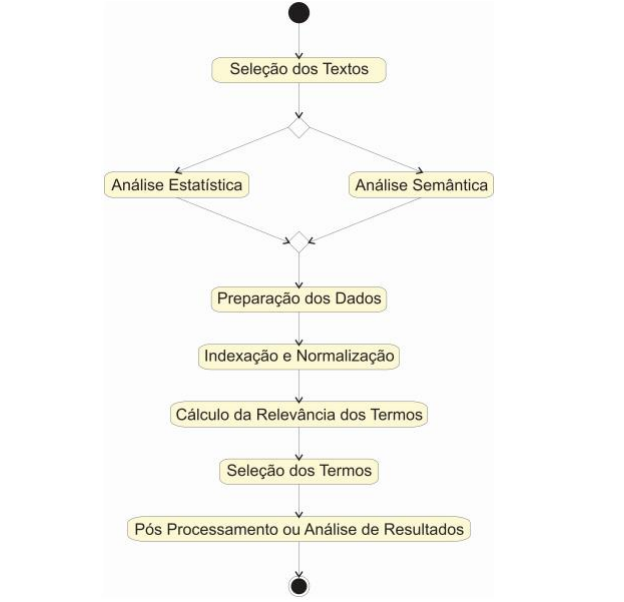
\includegraphics[scale=0.8]{figuras/figura_2.PNG} % altere o atributo scale para o tamanho da figura
	\end{center}
	\legend{Fonte: \cite{morais2007mineraccao}}
\end{figure}

\subsubsection{Abordagem dos dados}
\cite{morais2007mineraccao} apresenta dois tipos de abordagem dos dados textuais na área de mineração de textos: Análise Semântica, baseada na funcionalidade dos termos encontrados no texto, e Análise Estatística, baseada na frequência dos termos encontrados no texto. Estas abordagens podem ser utilizadas de forma separada ou em conjunto. A abordagem utilizada neste trabalho é a Análise Semântica.

\subsubsubsection{Análise Semântica}
Análise que avalia a sequência dos termos no texto sendo analisado, para identificar sua função, fundamentada em técnicas de \textit{Processamento de Linguagem Natural}. A análise semântica se dá pelo pelo conhecimento do significado das palavras de forma individual, independente do contexto, e também pelo conhecimento da estrutura dessas palavras, por exemplo, ao determinar os limites da palavra que determinam seu radical. A utilização de Análise Semântica se dá pela melhoria na qualidade dos resultados do processo de mineração de textos \cite{morais2007mineraccao}. 

Como as técnicas de análise semântica de textos procuram identificar a importância das palavras dentro da estrutura de orações \cite{morais2007mineraccao}, e por estar diretamente relacionada ao \textit{processamento de linguagem natural}, esse conceito é utilizado neste trabalho durante o pré-processamento dos dados, detalhado no Capítulo 5.


\subsubsection{Preparação dos dados}
A preparação dos dados envolve a seleção de dados que constituem a base de textos de interesse e o trabalho inicial para tentar selecionar o núcleo que melhor expressa o conteúdo desses textos. Além de prover uma redução dimensional, esta etapa procura identificar similaridades em função da morfologia ou do significado dos termos nos textos. O primeiro passo do processo de prepação dos dados é a \textit{Recuperação de Informação} \cite{morais2007mineraccao}. Um \textit{Sistema de Recuperação de Informação Textual} é um sistema desenvolvido para indexar e recuperar documentos do tipo textual. Nesse tipo de sistema as consultas são descritas através de termos e os documentos relevantes são recuperados de acordo com esses termos.

Outra etapa da preparação dos dados é a Análise de Relevância, onde o usuário pode entrar com um termo e obter como resposta um resultado de um problema em particular. A Análise de Relevância é utilizada principalmente para filtrar dados não pertencentes ao conjunto obtido. Essa etapa não é realizada, tendo em vista que os comentários coletados já compõem a base de dados desejada.

O ytCommentMiner \footnote{https://github.com/ssisaias/ytCommentMiner}, software desenvolvido para coleta dos comentários, é responsável pela etapa de preparação dos dados, até o momento da coleta dos textos online. A ferramenta não implementa a etapa de Análise de Relevância sobre o conjunto obtido.

\subsubsection{Indexação e Normalização}
O objetivo principal da indexação e normalização dos textos é facilitar a identificação de similaridade de significado entre suas palavras, considerando variações morfológicas e problemas de sinonímia \cite{morais2007mineraccao}. Este processo tem como resultado a geração de um índice, construído através de um processo de indexação. Um documento pode ser indexado por termos diferentes que são correspondentes ao vocabulário utilizado em sua área. Nesse caso, geralmente, há um conjunto de termos predefinidos e específicos para cada assunto da área em questão \cite{morais2007mineraccao}.

Em mineração de textos, a indexação é um processo automático. Suas principais fases são: \textit{identificação de termos} (simples ou composto); remoção de \textit{stopwords} (palavras irrelevantes); e \textit{normalização morfológica} (stemming) \cite{morais2007mineraccao}.

\begin{figure}[H] %use h para forçar que a figura fique abaixo do texto
	\caption{\label{fig:figura-4} Etapas do Processo de Indexação Automática}
	\begin{center}
	    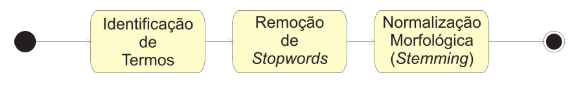
\includegraphics[scale=0.8]{figuras/figura_4.PNG} % altere o atributo scale para o tamanho da figura
	\end{center}
	\legend{Fonte: \cite{morais2007mineraccao}}
\end{figure}

A identificação dos termos consiste em identificar os termos contidos nos textos, sejam palavras simples ou termos compostos por duas ou mais palavras, também pode ser realizada uma correção dos erros gramaticais atravé de um dicionário de termos \cite{morais2007mineraccao}. 

Remoção de \textit{stopwords} consiste em eliminar palavras que não devem ser consideradas no documento, conhecidas como \textit{stopwords}. \textit{Stopwords} são palavras não relevantes ao texto, por não traduzirem sua essência. Normalmente fazem parte da lista de \textit{stopwords} preposições, pronomes, artigos, advérbios e outras classes de palavras auxiliares \cite{morais2007mineraccao}.

Também durante o processo de indexação, torna-se interessante remover as variações morfológicas de uma palavra, através da identificação do seu radical. Os prefixos e os sufixos são removidos, e apenas o radical resultante é adicionado ao índice. Essa técnica é chamada de lematização ou \textit{stemming} \cite{morais2007mineraccao}.

A identificação dos termos, remoção dos stopwords e \textit{steeming}, neste trabalho são realizados automaticamente através de \textit{scripts} e descritos no Capítulo 5.

\subsubsection{Cálculo de relevância dos termos}
Com exceção das \textit{stopwords}, os termos mais frequentemente utilizados no texto, costumam ter maior importância, assim como palavras constantes em títulos ou em outras estruturas, uma vez que foram colocadas ali por serem consideradas relevantes para a idéia do documento \cite{morais2007mineraccao}.

O cálculo de relevância de uma palavra em relação ao texto que está inserida pode se basear na frequência da mesma, na análise estrutural do documento, ou na posição sintática da palavra. Ao grau de relacionamento da palavra com o texto dá-se o nome de \textit{peso}. Logo é o peso que indica a importância da palavra em relação ao texto \cite{morais2007mineraccao}. 

\cite{morais2007mineraccao} apresenta algumas formas para cáculo do peso, que utilizam cálculos simples de frequência: \textit{frequência absoluta}, \textit{frequência relativa}, \textit{frequência inversa de documentos}. Nenhuma dessa técnicas é utilizada neste trabalho. Neste trabalho, o cálculo da relevância dos termos é realizado ao preparar o dicionário da ferramenta \textit{Sentistrength}, onde é possível dar um nível de relevância para cada palavra individualmente.

\subsubsection{Seleção dos termos}
Seleção de termos corresponde à etapa de seleção das palavras retiradas do texto, após os
processos de pré-processamento e cálculo da relevância. Esta técnica pode ser baseada no peso dos termos ou na sua posição sintática em relação ao texto. Entre as principais técnicas de seleção dos termos está a \textit{Seleção por análise de linguagem natural} \cite{morais2007mineraccao}, utilizada neste trabalho.

\subsubsubsection{Seleção por análise linguagem natural}
A \textit{seleção por análise de linguagem natural} consistem em aplicar técnicas de análise sintática ou semântica para identificar palavras em um documento. A análise semântica baseia-se no princípio de que as partes mais relevantes de um documento já estão de alguma forma demarcadas por estruturas de formatação específicas para isso \cite{morais2007mineraccao}.

A \textit{Seleção por análise de linguagem natural} é utilizada pelo autor tanto no momento da extração dos textos dos conjuntos de comentários obtidos, como durante a montagem do modelo de classificação, tendo em vista que há uma classificação prévia do grupo de treino dos comentários e uma triagem dos comentários classificados antes de serem utilizados para criação de fato do modelo.

\subsubsection{Pós processamento ou análise dos resultados}
Esta fase envolve a aplicação de técnicas de análise dos resultados de um Sistema de Recuperação de Informações de Texto, particularmente os resultados do processo de mineração de textos. A análise pode ser utilizada como forma de avaliação do \textit{Sistema de Recuperações de Informação de Texto}, para saber se funcionou como deveria ou não \cite{morais2007mineraccao}.

Entre as principais métricas de análise de \textit{Sistema de Recuperações de Informação de Texto} estão: \textit{recall} e \textit{precision}.

\subsubsubsection{\textit{Recall}}
O \textit{recall} (abrangência ou revocação) mede a habilidade do sistema em recuperar os documentos mais relevantes para seu usuário, com base no termo ou expressão utilizado na formulação de sua busca \cite{morais2007mineraccao}.

Sua fórmula consiste em:

\begin{equation}
\label{eq:recall-description-morais}
 {recall} = \frac{{n-recuperados-relevantes}}{{n-possiveis-relevantes}}, onde:
\end{equation}

n-recuperados-relevantes: é o número de documentos relevantes recuperados.

n-possíveis-relevantes: é o número total de documentos relevantes do sistema. Essa informação
geralmente não é conhecida e só pode ser estimada estatisticamente.

\subsubsubsection{\textit{Precision}}
A \textit{precision} (precisão) mede a habilidade do sistema em manter os documentos irrelevantes fora do resultado de uma consulta \cite{morais2007mineraccao}.

Sua fórmula consiste em:

\begin{equation}
\label{eq:precision-description-morais}
 {precision} = \frac{{n-recuperados-relevantes}}{{n-total-recuperados}}, onde:
\end{equation}

n-recuperados-relevantes: é o número de documentos relevantes recuperados.

n-total-recuperados: é o número total de documentos do sistema.


\subsection{Processamento de Linguagem Natural}
\cite{liddy2001naturallanguage} define \textit{Processamento de Linguagem Natural (Natural Language Processing - NLP)} como um conjunto de técnicas para analisar e representar textos de origem natural, em um ou mais níveis de análise linguística com o propósito de atingir processamento linguístico similar ao humano para um conjunto de tarefas ou aplicações. 

Para mineração de textos armazenados em formato não estruturados, são necessárias técnicas e ferramentas específicas da área de \textit{Descoberta de Conhecimento em Textos (Knowledge Discovery from Text - KDT)} \cite{morais2007mineraccao}. Para recuperação de informação, KDT e mineração de textos possuem alto grau de dependência de Processamento de Linguagem Natural.
% Na Seção, processamento em linguagem natural explicar a técnica NLP. Detalhar como ela é utilizada.
Neste trabalho, NLP é utilizada tendo em vista que o ato de interpretar e manipular palavras como parte de uma linguagem é considerado Processamento de Linguagem Natural \cite{morais2007mineraccao}.


\subsection{SentiStrength}
SentiStrength é um classificador léxico que utiliza regras de linguística para detectar a força de um sentimento em uma frase \cite{thelwall2012sentistrength}.

Para cada texto classificado, a ferramenta gera dois valores inteiros que variam de 1 a 5 numa escala positiva e 1 a 5 numa escala negativa, sendo o valor 1, um indicador de neutralidade para o sentimento. Por exemplo, uma classificação que retorna 3, 5 indica uma nota 3 para o sentimento positivo e nota 5 para o sentimento negativo, nesse caso o texto tem mais força negativa do que positiva \cite{thelwall2012sentistrength}.

O classificador SentiStrength foi concebido para ser utilizado com diversos idiomas, porém seu dicionário padrão é em inglês. É possível adaptar seu dicionário para outros idiomas. O dicionário utilizado pelo autor neste trabalho, parte de um dicionário português limitado que é fornecido no site da ferramenta SentiStrength, porém adaptado com mais palavrões e algumas correções, para uma detecção mais abrangente. A lista completa dos palavrões adicionados, assim como sua relevância na classificação é indicada no Apêndice B. O dicionário utilizado, em sua completude, pode ser encontrado no Apêndice A. Além disso, foi feito um script \footnote{https://gist.github.com/ssisaias/08b2c8494a4553612987c9d4ae94f86c} para converter a classificação gerada pela ferramenta, para a entrada esperada pelo classificador Naïve Bayes, essa etapa é descrita na seção de procedimentos.


\subsection{Naive Bayes}
Segundo \cite{tan2009DataMining}, uma técnica de classificação é uma maneira de construir modelos de classificação a partir de um \textit{Dataset}. Exemplos de classificadores são: Árvore de decisão; Rede Neurais; SVM (Support Vector Machines); e classificadores Naïve Bayes.
Cada uma dessas técnicas aplica um algoritmo de aprendizagem para identificar o modelo que melhor descreve um relacionamento entre o conjunto de atributos e as classes dos dados de entrada. Sendo assim o modelo gerado pelo algoritmo de aprendizagem deve ser capaz de, a partir de um conjunto de entradas, classificar corretamente registros que não eram conhecidos até então.

Naïve Bayes é um dos algoritmos mais eficientes para \textit{machine learning} e mineração de textos. Esse algoritmo de aprendizagem supervisionado utiliza do Teorema de Bayes, porém considerando haver independência entre as \textit{features} (característica das variáveis de entrada) do conteúdo sendo classificado \cite{zhang2004optimalitybayes}.

De acordo com com \cite{zhang2004optimalitybayes}, o Teorema de Bayes com \textit{features} dependentes pode ser definido da seguinte maneira, onde por exemplo, a probabilidade $P$ de um $comentario$ ser de classe $c$ é:

\begin{equation}
\label{eq:bayes_classic}
 P(c|comentário) = P(c) \frac{P(comentario |c)}{P(comentario)}
\end{equation}

Considerando existem duas classes, \textbf{positivo} e \textbf{negativo}, o evento $comentario$ pertence a classe $positivo$ se somente se:

\begin{equation}
\label{eq:bayes_classic}
 {f_b}(comentario) =  \frac{P(positivo| comentario)}{P(negativo| comentario)} \geq 1
\end{equation}

onde ${f_b}(comentario)$ é um classificador Bayesiano.

Ao assumir que as \textit{features} são independentes dados os valores de classe, ou seja:

\begin{equation}
\label{eq:naive_bayes}
 {p}(comentario|c) =  {p}({comentario_1, comentario_2, ..., comentario_n}|c) = \prod_{i=1}^{n} {p}(comentario_i|c),
\end{equation}

O classificador resultante é:

\begin{equation}
\label{eq:bayes_classic}
 {f_nb}(comentario) =  \frac{P(positivo)}{P(negativo)} \prod_{i=1}^{n} \frac{P({comentario_i} | positivo)}{P({comentario_i} | negativo)}
\end{equation}

A função ${f_nb}(comentario)$ é chamada de classificador Naive Bayes (Naïve Bayesian Classifier).


Neste trabalho é utilizada uma instância de Naïve Bayes chamada \textit{Multinomial Naïve Bayes}. \textit{Multinomial Naïve Bayes} indica que ${p}(comentario_i|c)$ possui uma distribuição multinomial. \textit{Multinomial Naïve Bayes} é altamente recomendado para processamento de texto não estruturado onde há contagem de palavras ao considerar a relevância dos termos \cite{metsis2006whichnaivebayes}.
A criação de um modelo Multinomial Naïve Bayes se dá através da ferramenta \textit{scikit-learn}, onde o processo de criação do classificador já é previamente implementado. \textit{scikit-learn} é uma biblioteca de aprendizagem de máquina desenvolvida na linguagem \textit{Python} \cite{scikit-learn}. 

